\subsection{Controlled simulation: projection geometry under distribution shift}

We evaluate the theory in a continuous-state offline RL benchmark that separates
Bellman incompleteness from off-policy distribution shift. The environment is a
nonlinear two-dimensional navigation problem with five actions, a goal basin,
and a decoy basin that attracts behavior data. A grid solve at $\tau=10^{-3}$
gives the reference $Q^\star_\tau$, target stationary distribution, and oracle
density ratios. We consider three behavior regimes---nearly on-policy, mild
shift, and severe shift with low effective sample size; details are in
Appendix~\ref{app:soft-fqi-simulation-details}.

We compare standard soft FQI, oracle stationary-weighted soft FQI, and
estimated stationary-weighted soft FQI using a deliberately Bellman-incomplete
linear state-action $Q$ class. For the estimated method, we fit the stationary
density ratio with a DICE-style saddle-point moment estimator: the ratio and
critic share an RBF-polynomial RKHS dictionary, and estimation is regularized by
targeting discounted stationary ratios with $\gamma_w=0.95$. Thus the estimated
method is a finite-dimensional approximation to the oracle stationary
reweighting. We use direct low-temperature fitting at $\tau=10^{-3}$; appendix
experiments repeat the annealing comparison at both $\tau=10^{-3}$ and the
near-hard-max value $\tau=10^{-6}$, where annealing changes median stationary
projected Bellman error by only $0.35$--$1.35\%$.

The main diagnostics are stationary projected Bellman error and
advantage-centered stationary $Q$ error. These directly test the local
stationary geometry predicted by the theory while ignoring raw $Q$ shifts that
are irrelevant for low-temperature action choice.

\begin{figure}[t]
\centering
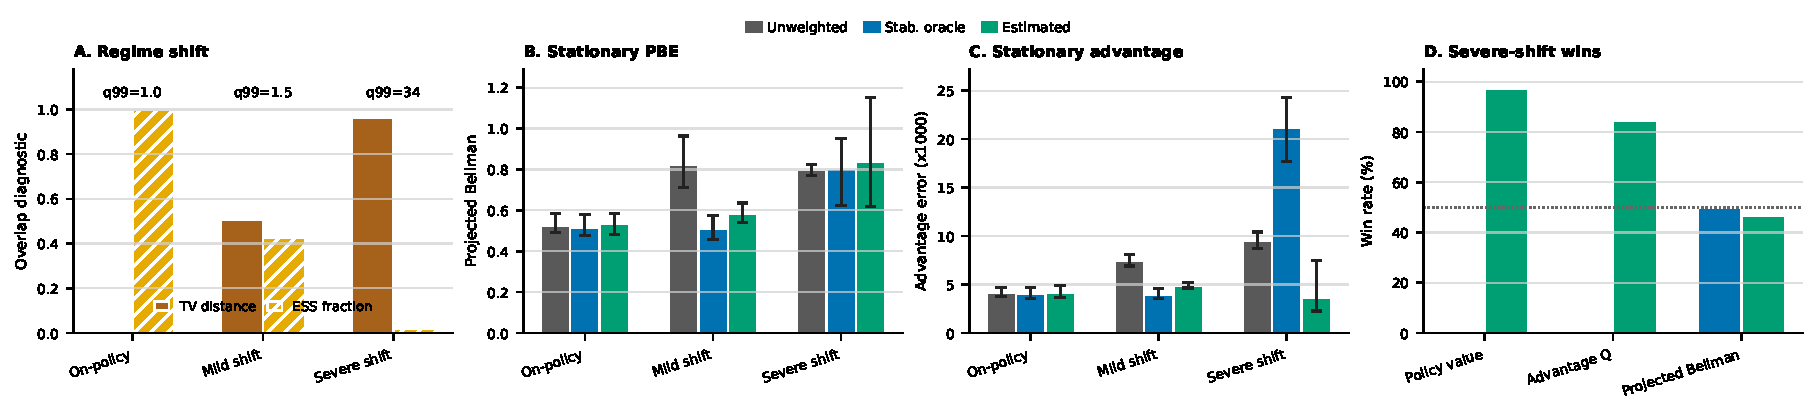
\includegraphics[width=0.5\linewidth]{final_draft_bundle/main_text_simulation_figure.pdf}
\caption{Controlled soft-FQI simulation. (A) Behavior regimes range from
nearly stationary to severe off-policy shift. (B) Stationary projected Bellman
error. (C) Advantage-centered stationary $Q$ error. (D) Severe-shift win rates.
Points and intervals in (B)--(C) are medians and IQRs over 200 datasets.}
\label{fig:soft-fqi-main}
\end{figure}

Figure~\ref{fig:soft-fqi-main} shows the intended pattern. In the on-policy
regime, weighting is neutral because the behavior norm already matches the
target stationary geometry. Under mild shift, unweighted soft FQI has much
larger target-stationary Bellman and advantage errors, while both oracle
weighting and the simpler estimated $\gamma_w=0.95$ weights recover most of the
loss. Thus, accurate oracle ratios are not necessary for the main effect:
regularized RKHS/DICE-style weights are sufficient to improve the projection
geometry when coverage is adequate. Under severe shift, the ratios are high
variance and no method uniformly dominates every metric. Oracle ratios improve
median stationary projected Bellman error but have wide variability, while
estimated weights beat unweighted FQI on advantage error in 169 of 200 seeds
and policy value in 194 of 200 seeds, but only 93 of 200 seeds for projected
Bellman error. Thus the simulation also shows the practical limitation:
finite-sample ratio estimation becomes limiting under severe shift.
